Solve Laplace's Equation $u_{xx} + u_{yy} = 0$ on the domain $\Omega = [0, 4] \times [0, 2]$ with the following
Dirichlet boundary conditions: 

\begin{align*}
u(x, 0) &= 0, \; u(x, 2) = 0 \\
u(0, y) &= 1, \; u(4, y) = 0
\end{align*}

\begin{solution}\ \\\\
  We begin by assuming a product solution, i.e., $u(x, y) = f(x)g(x)$. We substitute this solution into Laplace's 
  Equation to find:

  $$
  gf_{xx} + fg_{yy} = 0
  $$

  We divide each side by $fg$ to find:

  $$
  \frac{1}{f}f_{xx} + \frac{1}{g}g_{yy} = 0
  $$


  Since our boundary conditions with fixed $y$ are homogeneous, we expect a periodic solution for $g(y)$, and so we let:

  $$
  \frac{1}{f}f_{xx} = -\frac{1}{g}g_{yy} = \lambda^2
  $$

  Our $y$-dependent solutions to $g_{yy} + \lambda^2 g = 0$ are therefore given by:

  $$
  g_n(y) = a_n \cos{\left(\lambda_n y \right)} + b_n \sin{\left(\lambda_n y \right)}
  $$

  Our boundary condition $0 = u(x, 0) = f(x)g(0)$ implies $g(0) = 0$ and hence:

  $$
  0 = g_n(0) = a_n \cos{\left(0\right)} + b_n \sin{\left(0\right)} = a_n
  $$

  Similarly, $0 = u(x, 2) = f(x)g(2)$ implies
  
  $$
  0 = g_n(2) = b_n \sin{\left(2 \lambda_n\right)}
  $$

  and hence $\lambda_n = \frac{n \pi}{2}$. Our $y$-dependent solution is thus simply 
  $g(y) = b_n \sin{(\frac{n \pi y}{2})}$. Our $x$-dependent system is given by $f_{xx} - \lambda^2 f = 0$; solutions
  to this ODE take the form:\footnote{
    We shift in the $x$-direction by a factor of $L = 4$, since Laplace's equation is spatially-invariant.
  }

  $$
    f(x) = c_n \sinh{[\lambda_n (x-4)]} + d_n \cosh{[\lambda_n (x-4)]}
  $$

  Our boundary condition $0 = u(4, y) = f(4)g(y)$ implies that $f(4) = 0$; we substitute this into the above ODE 
  solution to find:

  $$
    0 = f(4) = c_n \sinh{[\lambda_n (4-4)]} + d_n \cosh{[\lambda_n (4-4)]} = d_n
  $$

  Next, we reindex by defining $\alpha_n \coloneqq c_n b_n$ and observe by the principle of superposition that our
  solution $u(x, y)$ takes the following form:

  $$
  u(x, y) = \sum\limits_{n=1}^{\infty} \alpha_n \sinh{\left[ \frac{n \pi (x - 4)}{2} \right]} \sin{\left(\frac{n \pi y}{2}\right)}
  $$

  We solve for $\alpha_n$ by utilizing our final boundary condition to find:

  $$
  1 = u(0, y) = \sum\limits_{n=1}^{\infty} \alpha_n \sinh{(-2n \pi)} \sin{\left(\frac{n \pi y}{2}\right)}
  $$

  To isolate each $\alpha_n$, we multiply both sides by $\sin{\left(\frac{m \pi y}{2}\right)}$ and integrate over our
  domain with respect to $y$. The left-hand side then becomes:

  \begin{align*}
    \int_{0}^{2}{1 \sin{\left(\frac{m \pi y}{2} \right)}} \; dy &= \frac{2}{m \pi} \left[-\cos{\left( \frac{m \pi y}{2} \right)}\right] \biggm\rvert_{0}^{2} \\
                                                               &= -\frac{2}{m \pi} [\cos{(m \pi) - 1}] \\
                                                               &= \begin{cases}
                                                                 \frac{4}{m \pi} &\; \text{ if } m \text{ is odd} \\
                                                                 0               &\; \text{ if } m \text{ is even}
                                                              \end{cases}
  \end{align*}

  Similarly, the right-hand side becomes:\footnote{
    With a little bit of analysis magic to allow us to interchange the sum and integrals.
  }

  \begin{align*}
    \int_{0}^{2}{\sum\limits_{n=1}^{\infty} \alpha_n \sinh{(-2n \pi)} \sin{\left(\frac{n \pi y}{2}\right)} \sin{\left(\frac{m \pi y}{2}\right)}} \; dy &= 
    \sum\limits_{n=1}^{\infty} \alpha_n \sinh{(-2n \pi)} \int_{0}^{2}{\sin{\left(\frac{n \pi y}{2}\right)} \sin{\left(\frac{m \pi y}{2}\right)}} \; dy  \\
    &= \sum\limits_{n=1}^{\infty} \alpha_n \sinh{(-2n \pi)} \left(\frac{2}{2} \delta_{mn} \right) \\
    &= \alpha_m \sinh{(-2m \pi)}.
  \end{align*}

  We solve for $\alpha_m$ to find:

  $$
  \alpha_m = \begin{cases}
    \frac{4}{m \pi \sinh(-2m \pi)} &\; \text{ if } m \text{ is odd} \\
    0               &\; \text{ if } m \text{ is even}
  \end{cases}
  $$

  Our full solution to this system is therefore:

  $$
  u(x, y) = \sum\limits_{n=1}^{\infty} \frac{4}{(2n - 1) \pi \sinh{\left[-2(2n - 1) \pi\right]}} \sinh{\left[ \frac{(2n - 1) \pi (x - 4)}{2} \right]} \sin{\left[\frac{(2n - 1) \pi y}{2}\right]}
  $$

  \ \\\\
  We plot an approximation to this solution below:

  \begin{figure}[h]
    \centering
    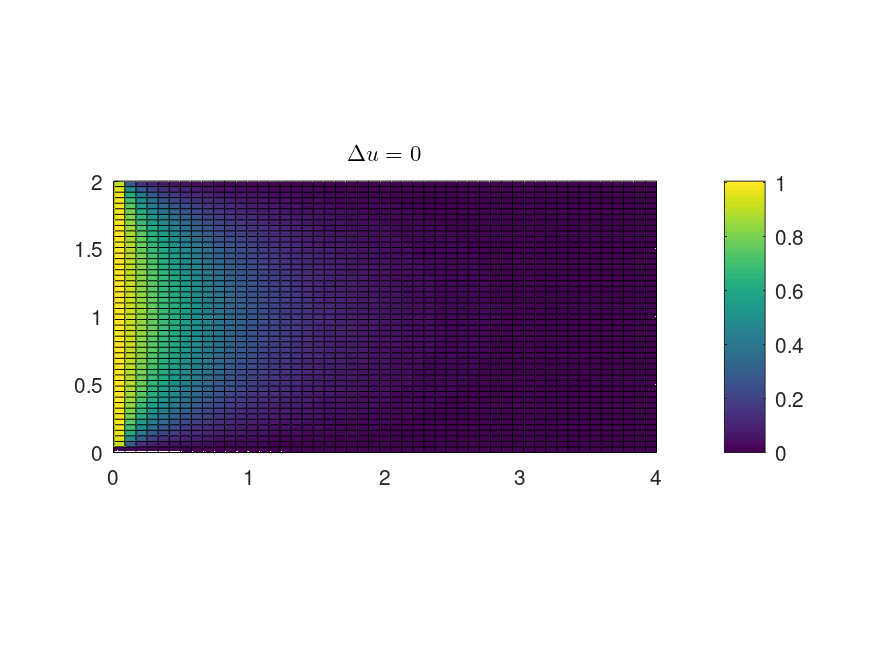
\includegraphics[width=\textwidth]{problem_1.png}
    \caption{First 100 solution terms to $\Delta u = 0$}
  \end{figure}

  \ \\
\end{solution}